\section{Deployment}

The deployment pipeline of the recommendation system involves setting up the Triton Ensemble and the external components of the system as shown in Figure \ref{fig:DeploymentDiagram}.
To use a Triton inference server, a Triton Ensemble has to be compiled with the necessary models, workflows, and configurations.

\subsection{Feast Materialization}

In order to use Feast as the feature store, the user and item features have to be materialized, 
meaning that they have to be moved from Feast's offline store, which in this case is a Parquet file, to its online store, which is a Redis database.

\subsection{Compiling Ensemble}

After the user and item features are materialized, the Triton Ensemble is compiled with all the models, workflows, and configurations.
Once compiled with all the components shown in Figure \ref{fig:DeploymentDiagram}, it outputs a directory tree similar to the one shown in Figure \ref{fig: EnsembleDirectoryTree}.

\begin{figure}[H]
    \centering
    \begin{subfigure}{.31\textwidth}
        \centering
        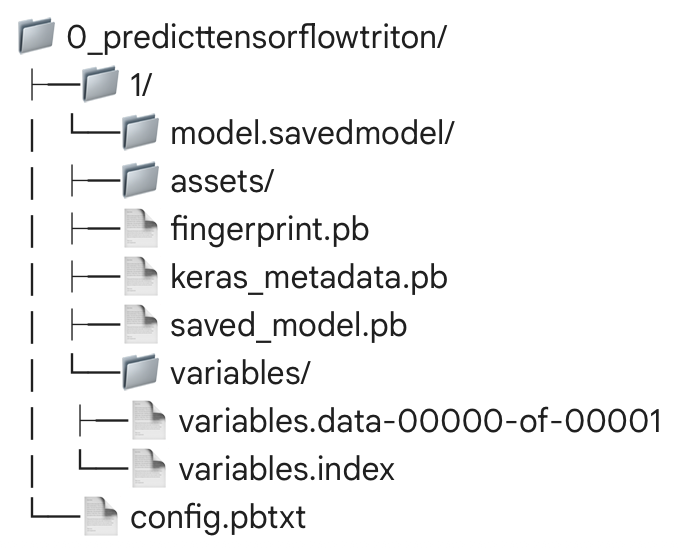
\includegraphics[width=\textwidth]{assets/ensemble_0.png}
        \label{fig:Ensemble0}
    \end{subfigure}
    \begin{subfigure}{.25\textwidth}
        \centering
        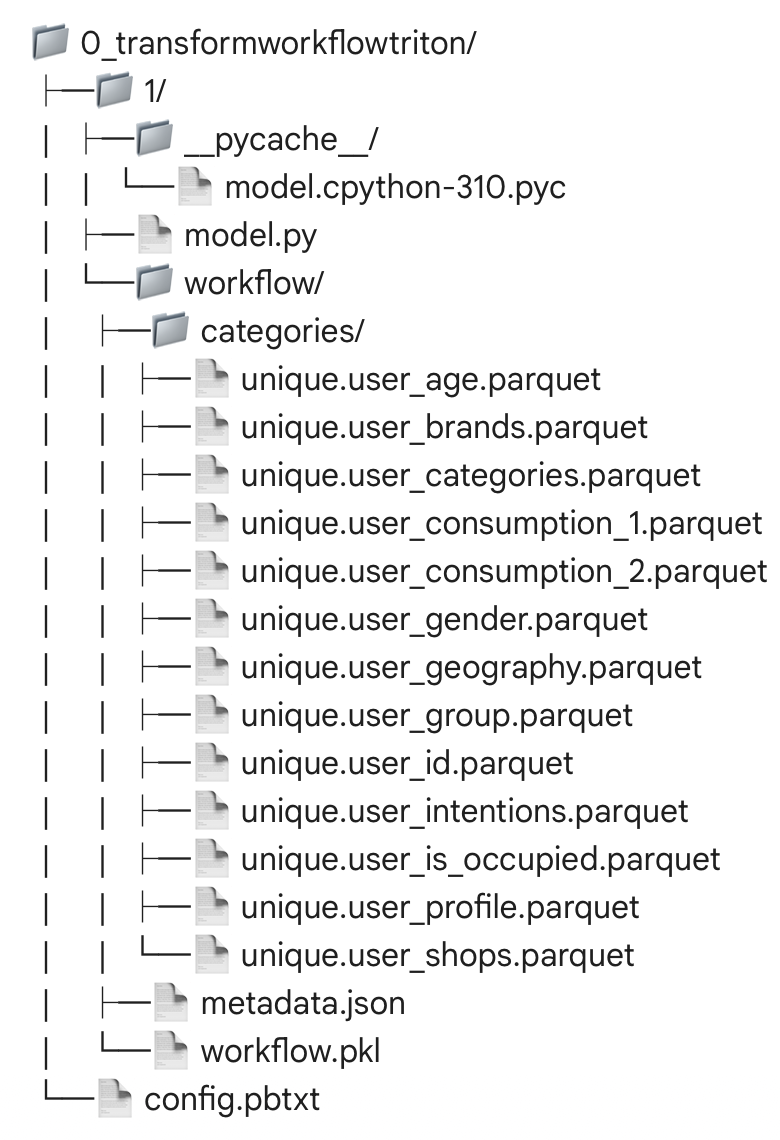
\includegraphics[width=\textwidth]{assets/ensemble_1.png}
        \label{fig:Ensemble1}
    \end{subfigure}
    \begin{subfigure}{.3\textwidth}
        \centering
        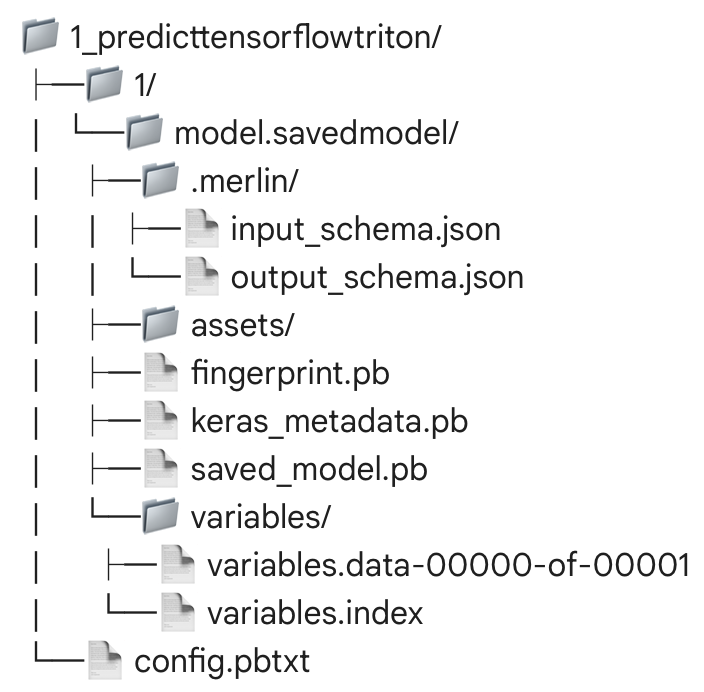
\includegraphics[width=\textwidth]{assets/ensemble_2.png}
        \label{fig:Ensemble2}
    \end{subfigure}
    \bigskip
    \begin{subfigure}{.3\textwidth}
        \centering
        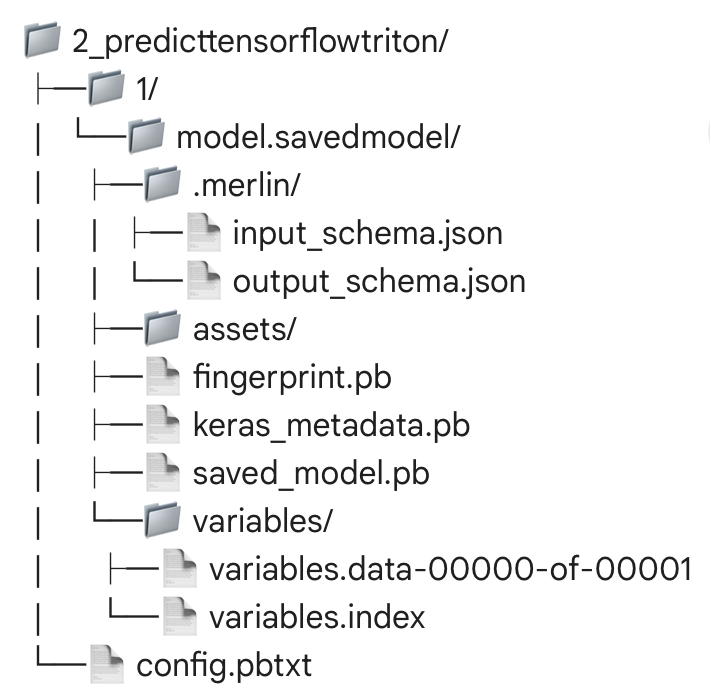
\includegraphics[width=\textwidth]{assets/ensemble_3.png}
        \label{fig:Ensemble3}
    \end{subfigure}
    \begin{subfigure}{.3\textwidth}
        \centering
        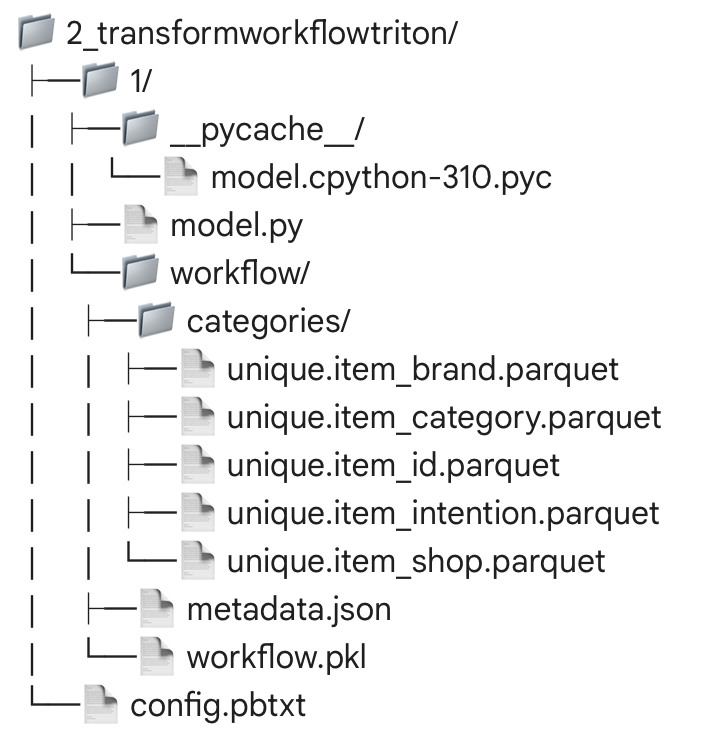
\includegraphics[width=\textwidth]{assets/ensemble_4.png}
        \label{fig:Ensemble4}
    \end{subfigure}
    \begin{subfigure}{.3\textwidth}
        \centering
        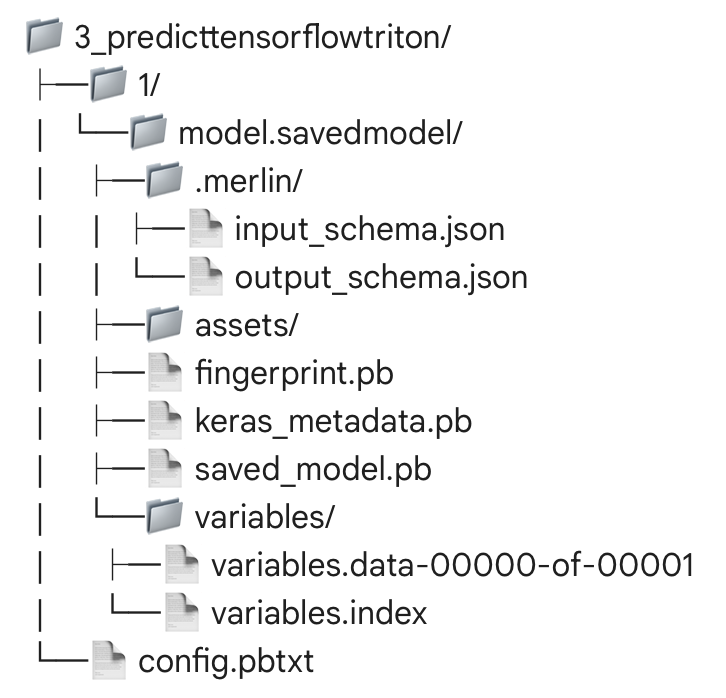
\includegraphics[width=\textwidth]{assets/ensemble_5.png}
        \label{fig:Ensemble5}
    \end{subfigure}
    \caption{Ensemble Directory Tree}
    \label{fig: EnsembleDirectoryTree}
\end{figure}


As shown in Figure~\ref{fig: EnsembleDirectoryTree}, the Triton Ensemble directory tree contains model configurations, model weights, embeddings categories, and other necessary files.
Those files are saved to the model repository.

\section{Demo}

Once the Triton Ensemble is compiled, the system can be deployed and tested.
When deploying a Triton Ensemble, by default, the Triton Inference Server is started on port 8001 for HTTP and 8002 for gRPC.
The Triton Inference Server can be accessed through the Triton Client, which is a Python library that allows the user to interact with the server.

A demo web UI was created to demonstrate the recommender system's functionality by illustrating its inputs and outputs.
To calculate metrics within the demo, a small subset of users with their positive clicks from the validation data was utilized.

The demo is a straightforward web application built using HTML, FastAPI~\cite{FastAPI}, and Tailwind CSS.
Figure~\ref{fig: Demo1} and Figure~\ref{fig: Demo2} show an illustrative example that represnts a sample input and output of the recommendation system.

Figure \ref{fig: Demo1} llustrates the recommendations generated for a specific user (ID \#12001) who has interacted with 306 items, representing the positive instances in the validation set.


\begin{figure}[H]
    \centering
    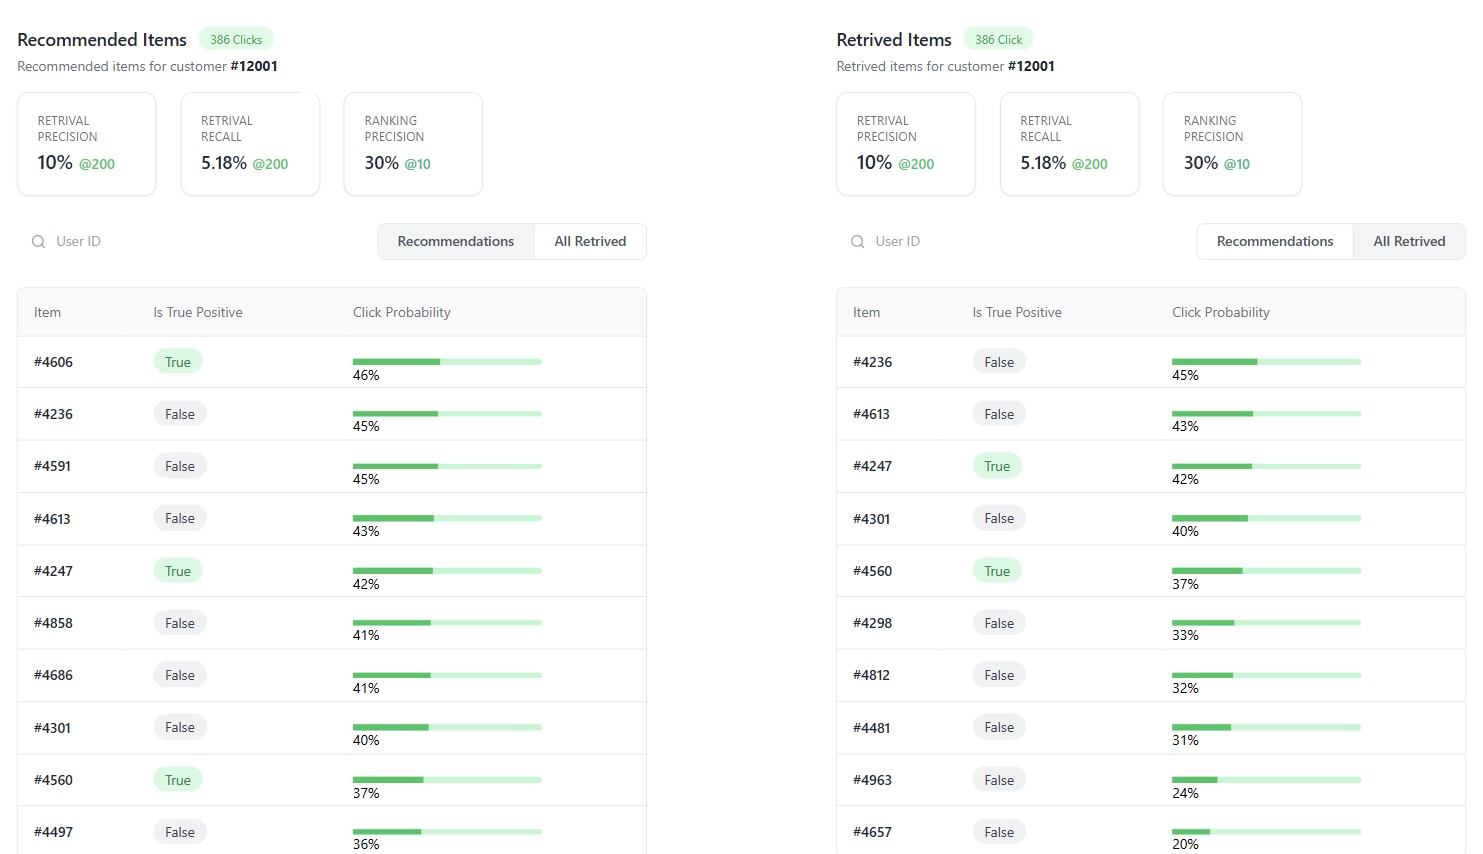
\includegraphics[width=\textwidth]{assets/demo_1.jpeg}
    \caption{Demo Example 1}
    \label{fig: Demo1}
\end{figure}

The left section displays the final 10 recommendations after Softmax sampling, each accompanied by its score. This list includes 3 true positives (items the user interacted with) and 7 false positives, resulting in a system precision of 30\%.

The right section lists all 200 items retrieved by the retrieval model, of which 20 are true positives and 180 are false positives. Based on these figures, the recall of the retrieval stage is calculated to be 5.18\% in this example.

Figure \ref{fig: Demo2} shows a different example, where the user (ID \#5042) has interacted with 57 items.

\begin{figure}[H]
    \centering
    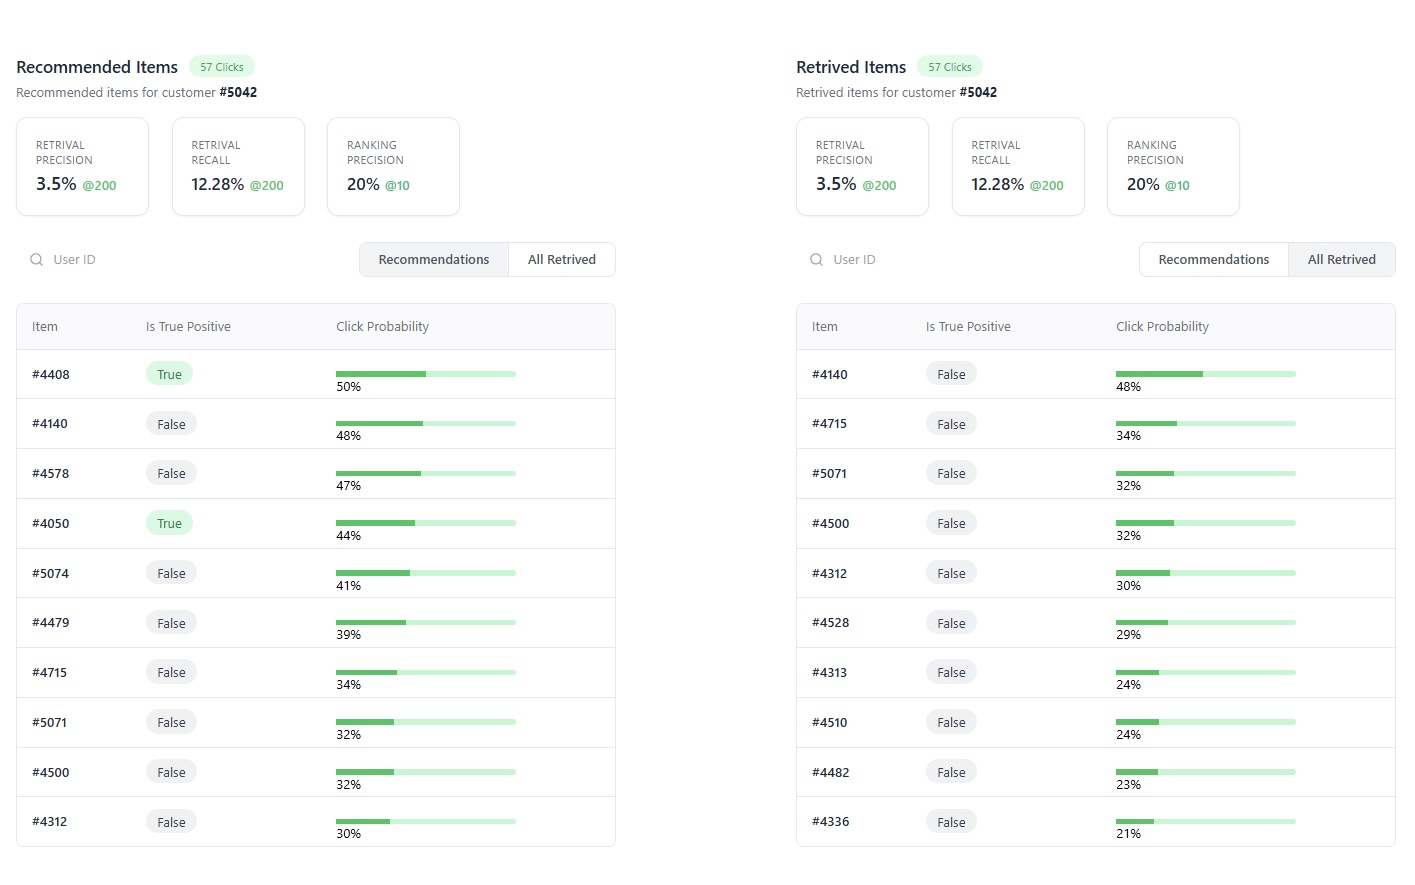
\includegraphics[width=\textwidth]{assets/demo_2.jpeg}
    \caption{Demo Example 2}
    \label{fig: Demo2}
\end{figure}

In the second example, the system was able to recommend 2 true positives in the final 10 recommendations, resulting in a precision of 20\%. 
The retrieval model retrieved 200 items, of which 7 were true positives, resulting in a retrieval recall of 12.28\%.


\section{Performance Evaluation}

To evaluate the performance of the recommendation system, a simple benchmark was conducted using the Triton Inference Client,
 100 request were sent to the server, and the average latency was calculated using different values for retrieval TopK items limit.

Figure \ref{fig:PerformanceEvaluation} shows the average latency of the system with different values for the TopK items limit.

\begin{figure}[H]
    \centering
    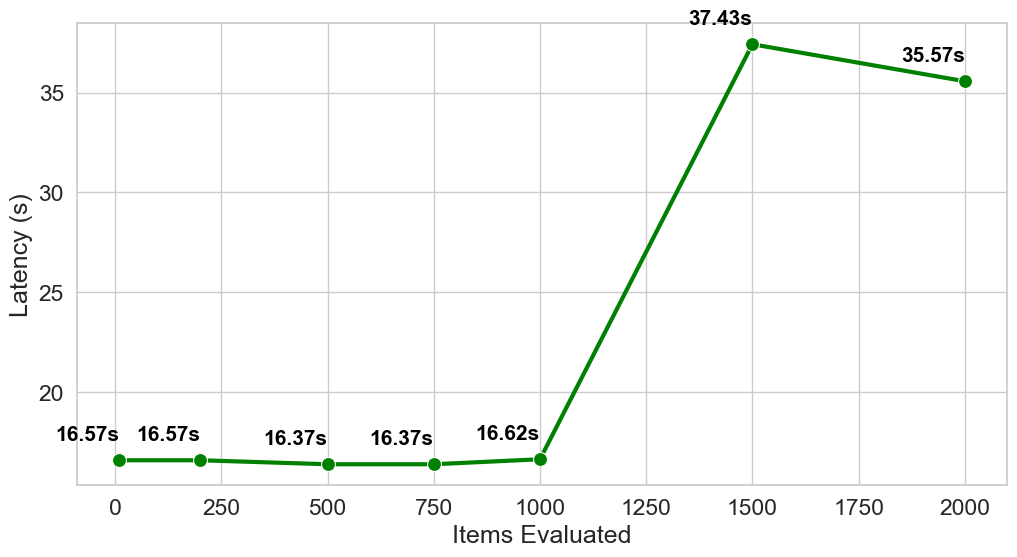
\includegraphics[width=\textwidth]{assets/performance_benchmark.png}
    \caption{Performance Evaluation}
    \label{fig:PerformanceEvaluation}
\end{figure}

As shown in Figure \ref{fig:PerformanceEvaluation}, the average latency of the system increases as the TopK items limit increases, this is because the bottle neck of the system is loading item features from the feature store, the more items are loaded the more time it takes to retrieve them.
Meanwhile the time required to evaluate 100 or 1000 item in the recommendation model is negligible compared to the time required to load the item features.

An approach to improve the performance of the system is to use a more efficient feature store, probably use a better offline store for Feast instead of Parquet files that are used in this experiment.


